\documentclass{beamer}
\usepackage{graphicx}
\usepackage{verbatim}
\usepackage{amsmath}
\usepackage{amsfonts}
\usepackage{setspace}
% \usepackage{beamerthemesplit} // Activate for custom appearance

\title{Regression Introduction and Estimation Review}
\author{Dr. Yang Feng}

\date{}

\DeclareMathOperator*{\Ave}{\mathbb{E}}
\DeclareMathOperator*{\Var}{Var}

\begin{document}

\frame{\titlepage}
\frame[t] {
 \frametitle{Formal Statement of Model}
$$Y_i = \beta_0 + \beta_1 X_i + \epsilon_i$$
\begin{itemize}
\item $Y_i$ value of the response variable in the $i^{th}$ trial
\item $\beta_0$ and $\beta_1$ are parameters
\item $X_i$ is a known constant, the value of the predictor variable in the $i^{th}$ trial
\item $\epsilon_i$ is a random error term with mean $\Ave(\epsilon_i)$ and variance
$\Var(\epsilon_i)=\sigma^2 $
\item $i = 1,\ldots,n$
\end{itemize}
}



\frame[t] {
 \frametitle{Least Squares Linear Regression}
\begin{itemize}
\item Seek to minimize $$Q = \sum_{i=1}^n (Y_i - (\beta_0 + \beta_1 X_i))^2$$
\item By careful choice of $b_0$ and $b_1$ where $b_0$ is a point estimator for $\beta_0$ and $b_1$ is the same for
$\beta_1$\\
How?

\end{itemize}
}

\frame[t] {%%%change pic%%%
 \frametitle{Guess \#1}
\begin{figure}
  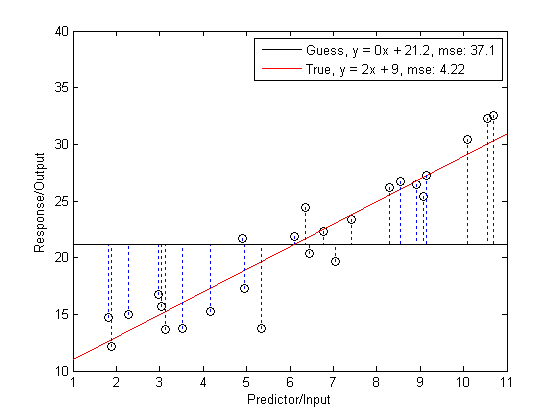
\includegraphics[height=60mm]{g1.png}
\end{figure}
}

\frame[t] {%%%change pic%%%
 \frametitle{Guess \#2}
\begin{figure}
  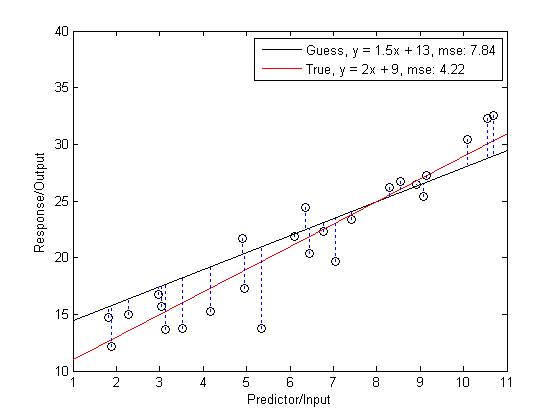
\includegraphics[height=60mm]{g2.png}
\end{figure}
}

\frame[t] {
 \frametitle{Function maximization}
\begin{itemize}
\item Important technique to remember!
\begin{itemize}
\item Take derivative
\item Set result equal to zero and solve
\item Test second derivative at that
point
\end{itemize}
\item Question: does this always give you the maximum?
\item Going further: multiple variables, convex optimization
\end{itemize}
}

\frame[t] {%%%change pic%%%
 \frametitle{Function Maximization}
Find the maximum value of x that satisfies the function $$-x^2 +
ln(x) = a, x>0$$
\begin{figure}
  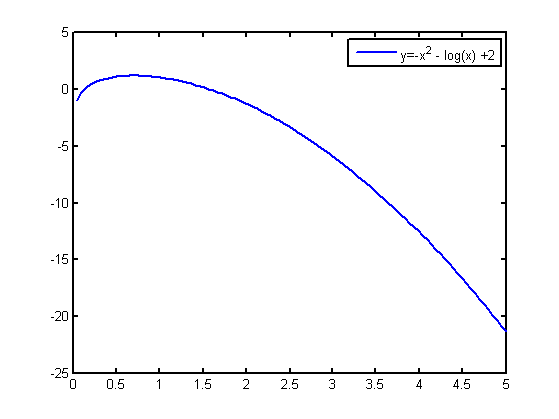
\includegraphics[height=60mm]{fmax.png}
\end{figure} }

\frame[t] {
 \frametitle{Least Squares Max(min)imization}
\begin{itemize}
\item Function to minimize w.r.t. $b_0$ and $ b_1$ -- $b_0$ and $b_1$ are called point estimators of $\beta_0$ and $\beta_1$ respectively
$$Q = \sum_{i=1}^n (Y_i - (b_0 + b_1 X_i))^2$$
\item Minimize this by maximizing -Q

\item Either way, find partials and set both equal to zero
\begin{eqnarray*}
\frac{dQ}{db_0} &=& 0 \\
\frac{dQ}{db_1} &=& 0
\end{eqnarray*}

\end{itemize}
}

\frame[t] {
 \frametitle{Normal Equations}
\begin{itemize}
\item The result of this maximization step are called the normal equations.
\begin{eqnarray*}
\sum Y_i &=& nb_0 + b_1 \sum X_i \\
\sum X_iY_i &=& b_0 \sum X_i + b_1 \sum X_i^2
\end{eqnarray*}

\item This is a system of two equations and two unknowns.  The solution is given
by$\ldots$

\end{itemize}
}

\frame[t] {
 \frametitle{Solution to Normal Equations}
After a lot of algebra one arrives at
\begin{eqnarray*}
b_1 &=& \frac{\sum(X_i - \bar X)(Y_i - \bar Y)}{\sum(X_i-\bar X)^2} \\
b_0 &=& \bar Y - b_1 \bar X\\
\bar X &=& \frac{\sum X_i}{n} \\
\bar Y&=&\frac{\sum Y_i}{n}
\end{eqnarray*}

}


\end{document}
